%%%%%%%%%%%%%%%%%%%%%%%%%%%%%%%%%%%%%%%%%
% Short Sectioned Assignment
% LaTeX Template
% Version 1.0 (5/5/12)
%
% This template has been downloaded from:
% http://www.LaTeXTemplates.com
%
% Original author:
% Frits Wenneker (http://www.howtotex.com)
%
% License:
% CC BY-NC-SA 3.0 (http://creativecommons.org/licenses/by-nc-sa/3.0/)
%
%%%%%%%%%%%%%%%%%%%%%%%%%%%%%%%%%%%%%%%%%

%----------------------------------------------------------------------------------------
%	PACKAGES AND OTHER DOCUMENT CONFIGURATIONS
%----------------------------------------------------------------------------------------

\documentclass[paper=a4, fontsize=11pt]{scrartcl} % A4 paper and 11pt font size

\usepackage[T1]{fontenc} % Use 8-bit encoding that has 256 glyphs
\usepackage{fourier} % Use the Adobe Utopia font for the document - comment this line to return to the LaTeX default
\usepackage[english]{babel} % English language/hyphenation
\usepackage{amsmath,amsfonts,amsthm} % Math packages

\usepackage{lipsum} % Used for inserting dummy 'Lorem ipsum' text into the template

\usepackage{sectsty} % Allows customizing section commands
\allsectionsfont{\centering \normalfont\scshape} % Make all sections centered, the default font and small caps

\usepackage{fancyhdr} % Custom headers and footers
\pagestyle{fancyplain} % Makes all pages in the document conform to the custom headers and footers
\fancyhead{} % No page header - if you want one, create it in the same way as the footers below
\fancyfoot[L]{} % Empty left footer
\fancyfoot[C]{} % Empty center footer
\fancyfoot[R]{\thepage} % Page numbering for right footer
\renewcommand{\headrulewidth}{0pt} % Remove header underlines
\renewcommand{\footrulewidth}{0pt} % Remove footer underlines
\setlength{\headheight}{13.6pt} % Customize the height of the header

\numberwithin{equation}{section} % Number equations within sections (i.e. 1.1, 1.2, 2.1, 2.2 instead of 1, 2, 3, 4)
\numberwithin{figure}{section} % Number figures within sections (i.e. 1.1, 1.2, 2.1, 2.2 instead of 1, 2, 3, 4)
\numberwithin{table}{section} % Number tables within sections (i.e. 1.1, 1.2, 2.1, 2.2 instead of 1, 2, 3, 4)

\setlength\parindent{0pt} % Removes all indentation from paragraphs - comment this line for an assignment with lots of text
\usepackage{graphicx}

%----------------------------------------------------------------------------------------
%	TITLE SECTION
%----------------------------------------------------------------------------------------

\newcommand{\horrule}[1]{\rule{\linewidth}{#1}} % Create horizontal rule command with 1 argument of height

\title{	
\normalfont \normalsize 
\textsc{University of Massachusetts Amherst- Computer Science-Fall 2013} \\ [25pt] % Your university, school and/or department name(s)
\horrule{0.5pt} \\[0.4cm] % Thin top horizontal rule
\huge JSProf: A Javascript Profiler \\ % The assignment title
\horrule{2pt} \\[0.5cm] % Thick bottom horizontal rule
}

\author{Authors: Eswer Kishore Kumar, Nimish Gupta} % Your name

\date{October 21,2013} % Today's date or a custom date

\begin{document}

\maketitle % Print the title

%----------------------------------------------------------------------------------------
%	PROBLEM 1
%----------------------------------------------------------------------------------------

\section{Introduction}

The aim of this project is to build a Javascript profiler written in Javascript. It is supposed to be browser independent. The profiler is expected to report the following information

%------------------------------------------------

\begin{enumerate}
\item Execution times for individual functions
\item Edges between caller and callee functions 
\item Frequency of calls
\item Reconstruction of the dynamic call paths
\item Identification of hot paths 
\item Tracking sources/causes of asynchronous callbacks
\end{enumerate}

%----------------------------------------------------------------------------------------
Original problem statement can be found at: http://plasma.cs.umass.edu/emery/grad-systems-project-1 

%------------------------------------------------

\section{Approach}
The basic flow of our application is like this. Individual stages are discussed in detail later.

Instrument code --> Collect Run Time data --> Post Process --> Show Results

\section{Instrument Code}
To collect the required information we need to have our special instructions in specific places in code. To collect and show the above information we need to track each function entry and function exit. For tracking asynchronous callbacks we need to look for call expressions in Javascript code. To capture function declarations and expressions in Javascript we first represent it into an annotated canonical form using a Javascript parser. We then traverse the canonical form to look for function declarations and function expressions and add our code to all functions found upon traversal. We use Esprima (http://esprima.org/) parser and Escodegen (https://github.com/Constellation/escodegen) to accomplish parsing and rewriting respectively.

Since a function can have multiple exit points, we wrap the function code into try finally block to ensure that we successfully capture function exit event.

Ex : Before instrumentation
       
        function () 
        
        {
                       
          <body>
        
        }
         
        After instrumentation

        function ()
        
        {
          capturefunctionentry ();
          
        }

        try 
         
        {
        
          <try block>
          
        } 
        
        finally
        
        {
        
          capturefunctionexit ();
          
        }
       

\section{Collect Run Time Information}

At run-time, the actual code interacts with our code that captures the run time call stack information. Since we are interested in capturing the time of function execution it is imperative that the overhead of our instrumentation code be minimal. We have taken various measures to ensure that this is the case. We collect call function call information on an array and tag it with start and stop time. The call stack information gives us edges between callers and callees, the time of execution of the edge and the number of times the call was made. As the program executes this data if not processed could easily occupy a lot of memory over a small interval of time. A program consists of fixed functions that are called arbitrary number of times. So reducing the callstack into edge information helps keep the memory overhead low. Since this will incur overhead if done in real-time so with do it asynchronously at a later stage.  We rely on the fact that Javascript programs are mostly asynchronous to keep our memory footprint low.

\section{Post Process}

All the data we have collected, needs to be passed to be processed for results. Our post processor takes the collection of edges as inputs and forms a graph out of it, propagating the times from edges to nodes.
We have taken care of self-recursion. The resulting data structure has the following information

For every function in graph we have the following information.

\begin{enumerate}
\item Its caller functions (parents)
\item Children
\item Total time in ms
\item Self time in ms
\item Number of  calls made to this function
\item Number of self recursive calls made
\end{enumerate}

The data is presented in a tree-tabular format. We present two views to the user.

\begin{enumerate}
\item Top Down View
\item Bottom Up View
\end{enumerate}

Top Down View: Top down view traces the execution flow of program, starting from the Javascript Engine context. The hot-path is highlighted with a distinct color. Initially the whole tree-table is collapsed to one single node. When expanded, it shows the functions which were called from the clicked function. The functions can be further clicked to know their children until we encounter a leaf node.

Bottom Up View: Bottom up view shows the list of functions along with their individual statistics. The functions comprising the hot-path are again highlighted. Upon clicking a function the tree expands to show the functions that calls the function that was clicked. This can be traced until we encounter the JS Engine context.

We have used a third party library called JQuery and JQuery tree-table to help us with the display of collapsible tree-table.

\section{System Design}
\subsection{Proxy Server}
A web page can have embedded JS and link to script files. We want the instrumentation to be transparent to the user. We have written a proxy program in node js that intercepts http requests. Instruments JS files before we send it to user. It also embeds link to our modules that collects and process the run-time data. This is done in the <head> tag to make sure that the modules are available before any JS code starts executing on the web page

\subsection{Web Interface}
We ask the user to enter the URL which he would like to profile, make the request to the web-page (through proxy server). We use an Iframe based UI to open the source page for user to interact with it. On top of the page we have a button that shows the user the result of execution. Since the pages are cross domain. We use message passing to communicate with our embedded module in the Iframe to pass the requests and profiling data for post processing.

\subsection{Testing}
Almost all the modules have been developed in node js compatible JS, but they don't use any node specific feature. Since proxy is server side thing we have used written it entirely in node. Additionally we are using the browserify (http://browserify.org/) module of node to convert the node modules to browser side JS. We have tested the individual modules in node using the few benchmarks (http://benchmarksgame.alioth.debian.org). Browser side testing was done with Chrome and Firefox.

\section{Results}
We are able to collect the required information and show it except that we are currently not tracing asynchronous callbacks. There is a slight overhead incurred while running the instrumented programs. We have been using http://esprima.org/demo/functiontrace.html as our reference and we have generally observed that the overhead involved is ~15-20%. The memory overhead is slightly high as we would have liked it to be. Some snapshots of results are given below

\begin{figure}[ht!]
\centering
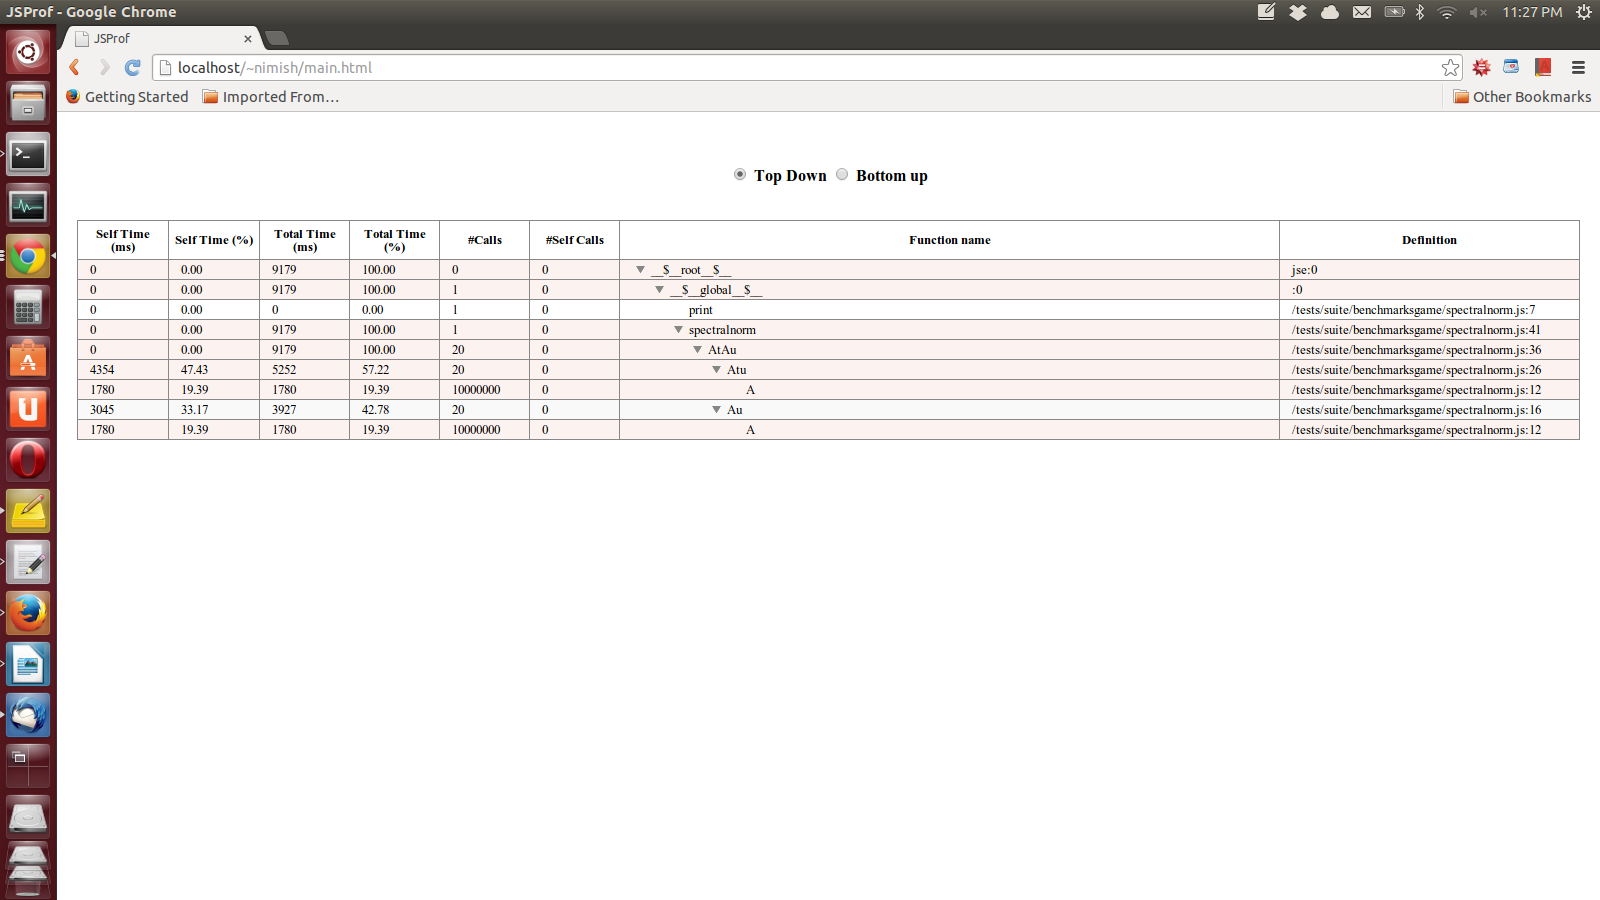
\includegraphics[width=150mm]{1.png}
\caption{Top Down View}
\label{overflow}
\end{figure}

\begin{figure}[ht!]
\centering
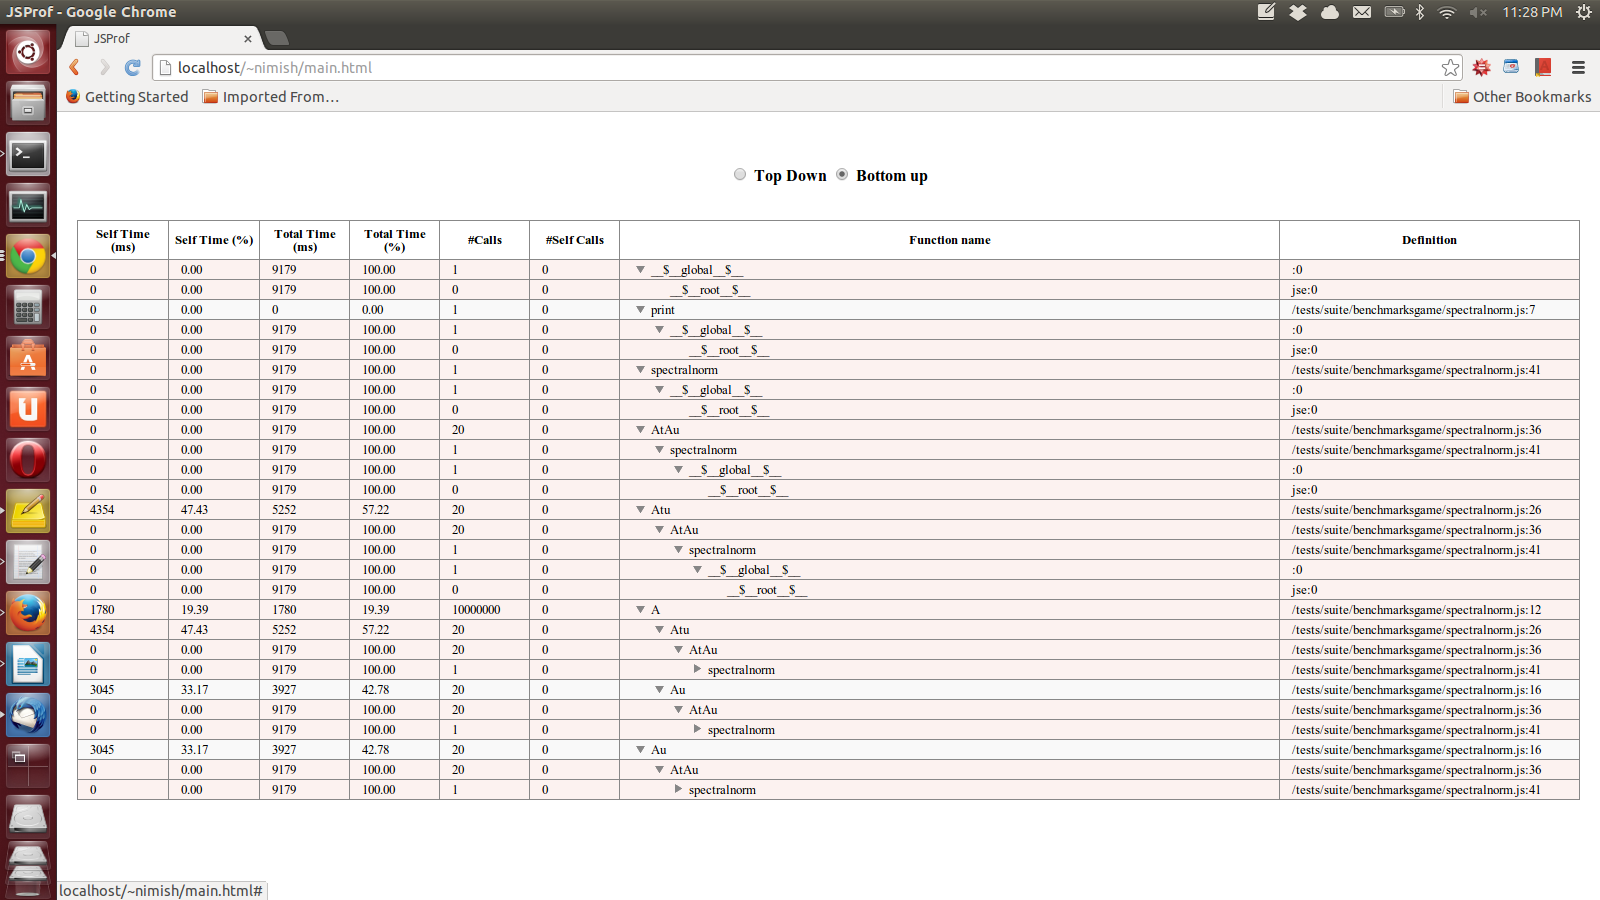
\includegraphics[width=150mm]{2.png}
\caption{Bottom Up View}
\label{overflow}
\end{figure}

\section{References}

\begin{enumerate}
\item Esprima JS Parser (http://esprima.org/)
\item Escodegen (https://github.com/Constellation/escodegen) 
\item Jquery (http://jquery.com/)
\item Jquery tree-table (http://plugins.jquery.com/treetable/)
\item Node (http://nodejs.org/) 
\item Browserify (http://browserify.org/)
\item Test Benchmarks ( http://benchmarksgame.alioth.debian.org)
\item Esprima function trace ( http://esprima.org/demo/functiontrace.html)
\end{enumerate}


\end{document}